\documentclass[sigplan,screen]{acmart}


\settopmatter{printacmref=false}
\setcopyright{none}
\renewcommand\footnotetextcopyrightpermission[1]{}
\pagestyle{plain}


\begin{document}


\title{Zero Trust Cellular Architecture on 5G}


\author{Changhao Zhao}
\email{changhaozhao@umass.edu}
\affiliation{%
  \institution{University of Massachusetts Amherst}
  \department{Department of Electrical and Computer Engineering}
  \city{Amherst}
  \state{Massachusetts}
  \country{USA}
}

\author{Hengyi Zhu}
\email{hengyizhu@umass.edu}
\affiliation{%
  \institution{University of Massachusetts Amherst}
  \department{Department of Electrical and Computer Engineering}
  \city{Amherst}
  \state{Massachusetts}
  \country{USA}
}

\author{Junfei Zhang}
\email{junfeizhang@umass.edu}
\affiliation{%
  \institution{University of Massachusetts Amherst}
  \department{Department of Electrical and Computer Engineering}
  \city{Amherst}
  \state{Massachusetts}
  \country{USA}
}


%%
%% The abstract is a short summary of the work to be presented in the
%% article.
\begin{abstract}
  As 5G networks proliferate globally, enhancing bandwidth and reducing latency, they also amplify challenges related to user privacy and data security. This paper introduces a Zero Trust Architecture (ZTA) for 5G networks, which mandates rigorous authentication and authorization for each access request, thereby enhancing security against complex cyber threats. We detail the design and implementation of a 5G cellular system that uses Globally Unique Temporary Identifiers (GUTIs) to pseudonymize user identities, thus safeguarding privacy without inherent trust in network components. The system's effectiveness is validated through experiments, with discussions on future enhancements for 5G security.
\end{abstract}


\keywords{5G Networks, Zero Trust Architecture, Data Security, Network Access Control, Globally Unique Temporary Identifier}


\maketitle

\section{Introduction}

The advent of 5G technology has heralded unprecedented improvements in communication speed, capacity, and connectivity, enabling the rapid expansion of Internet of Things (IoT) applications and smart city infrastructures. However, these advancements also introduce significant vulnerabilities in user privacy and data security, exacerbated by the inherent open and decentralized nature of these networks. Traditional trust-based security models, reliant on established perimeters and internal trust zones, are increasingly inadequate for addressing the dynamic and heterogeneous threats faced by modern mobile networks. This has led to an urgent need to enhance user privacy protections while maintaining network efficiency, particularly in light of sophisticated network attacks, often targeting mobile devices.

In response to these challenges, this paper advocates for the adoption of ZTA within 5G frameworks, a paradigm shift in network security that eliminates implicit trust and requires strict verification of every access request, regardless of the entity's location within or outside the network. ZTA addresses both insider threats and external attacks more effectively by enforcing strict access controls and minimal privilege access.

The primary motivation for integrating ZTA into 5G networks arises not only from these security challenges but also from the pervasive expansion of tracking technologies. Websites and third-party trackers capture extensive user web browsing activities, often linking user activities to data profiles for purposes like fraud prevention and targeted advertising. Yet, the boundary between legitimate data collection and privacy infringement remains ambiguous. This challenge is compounded in 5G networks, where traditional defenses like cookie management are less effective against implicit tracking methods such as those utilizing Globally Unique Temporary Identifiers (GUTIs).

To practically implement ZTA, this study introduces a system that uses GUTIs to anonymize user identities, thereby enhancing privacy without trusting any network component. The system not only protects user data but also integrates seamlessly with the dynamic and scalable nature of 5G technologies. The design and implementation of this system are detailed, followed by a discussion of the experimental validation of its effectiveness.

Through rigorous analysis and empirical testing, this paper demonstrates the feasibility and benefits of integrating ZTA into 5G networks, providing a robust framework for securing next-generation telecommunications against evolving cyber threats. We also outline the detailed design and implementation process of the system, explore the relevant background knowledge on 5G network architecture and Zero Trust Architecture, and propose potential future directions for enhancing privacy and security in 5G networks.


\section{Background}
In this section, we review the cellular network architecture and the associated identities and procedures relevant to location privacy and data security within 5G networks.

\subsection{Overview of 5G Cellular Network Architecture}

\begin{figure}[htbp]
\centering
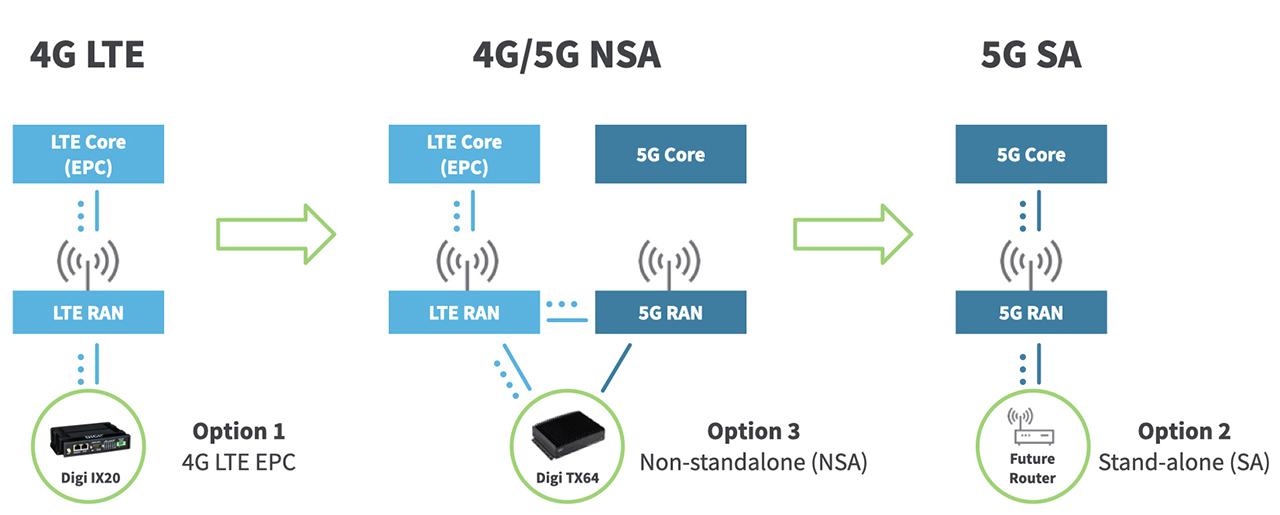
\includegraphics[width=\linewidth]{5gMigration.jpg}
\caption{The migration of 5G network infrastructure. (\url{https://www.digi.com/blog/post/5g-network-architecture}).}
\Description{The migration of 5G network infrastructure.}
\end{figure}

The architecture of 5G networks consists of three primary components: the Core Network, Access Network, and User Equipment (UE). The Core Network acts as the hub, managing connectivity, mobility, session handling, and data routing. The Access Network, made up of multiple base stations, communicates with user devices such as smartphones and IoT devices via radio signals.

Communication between the Access Network and Core Network in 5G systems is facilitated by the 5G Radio Access Network (5G-RAN), which supports advanced technologies like millimeter waves (mmWave) and Massive Multiple Input Multiple Output (Massive MIMO). These technologies provide high bandwidth and improved signal efficiency and coverage, enabling reliable, high-speed connections in densely populated areas, although the network still requires centralized management.

The 5G Core Network uses a Service-Based Architecture (SBA) that enhances flexibility and scalability by decomposing core functions into independent Network Functions (NFs). This setup allows for dynamic resource allocation based on demand.

UE includes devices that connect and communicate with the network. The Radio Access Network (RAN) consists of base stations known as eNodeBs, which manage service areas called "Cells." A group of these cells forms a "Tracking Area" (TA), identified by a unique Tracking Area Code (TAC). The Mobility Management Entity (MME) uses the TAC and MME code (MMEC) to track subscriber locations. \cite{hong2018guti}

The workflow within a 5G network typically operates as follows:

\begin{figure}[htbp]
\centering
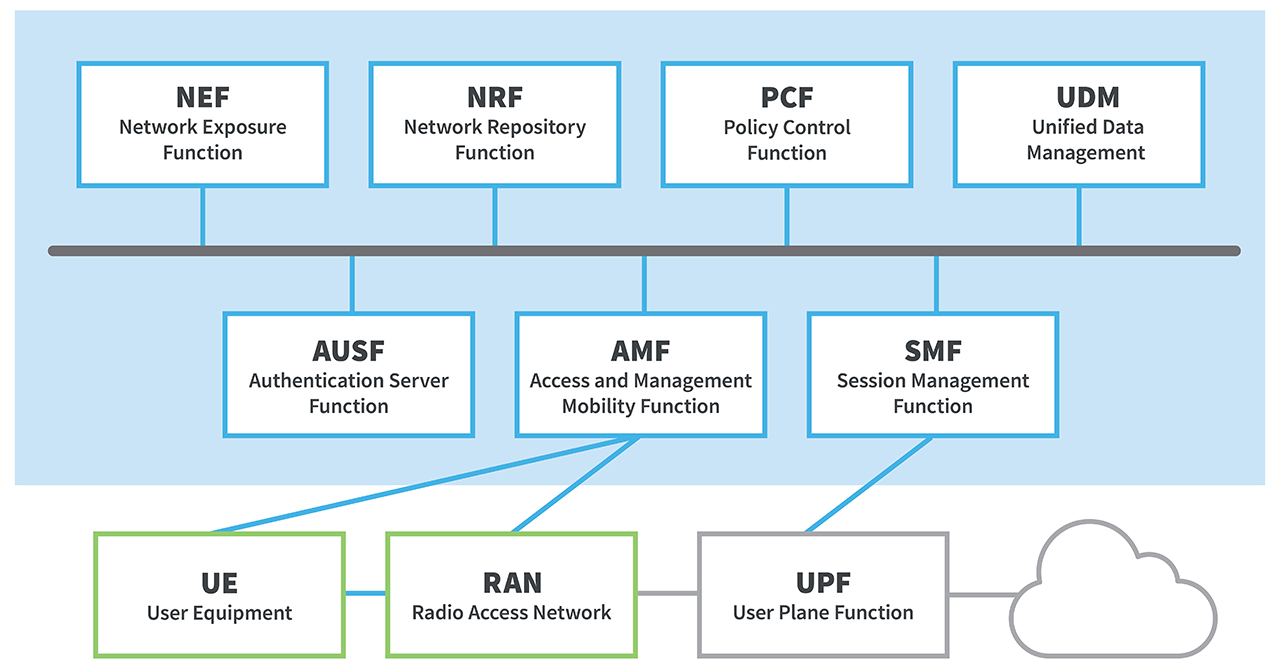
\includegraphics[width=\linewidth]{5gArchitecture.jpg}
\caption{The 5G network topology diagram shows the key components of a 5G core network. (\url{https://www.techplayon.com/5g-reference-network-architecture/}).}
\Description{The 5G network topology diagram shows the key components of a 5G core network.}
\end{figure}

\begin{itemize}
\item UE, such as a 5G smartphone or 5G cellular device, connects to the 5G core network via the 5G New Radio Access Network and subsequently to data networks (DN) such as the internet.
\item The Access and Mobility Management Function (AMF) serves as the single entry point for the UE's connection. 
\item  Based on the service requested by the UE, the AMF selects the appropriate Session Management Function (SMF) to manage the user's session.
\item The User Plane Function (UPF) facilitates the transmission of IP data streams (user plane) between the UE and external networks.
\item The Authentication Server Function (AUSF) allows the AMF to authenticate the UE and access services within the 5G core.
\item Other functions such as the SMF, Policy Control Function (PCF), Application Function (AF), and Unified Data Management (UDM) function provide policy control frameworks, application policy decisions, and access to subscription information to manage network behavior.
\end{itemize}


\subsection{Zero-Trust Architecture}
Although 5G networks introduce several decentralized design concepts such as distributed computing and edge computing, the overall architecture still retains centralized control through the core network. The 5G cellular network architecture, with its advanced technologies and design, achieves significant performance enhancements and supports a diverse array of applications. However, as network openness and decentralization increase, effectively protecting user privacy and data security remains a critical challenge. The zero-trust model offers an effective solution to these issues. \cite{ahmadi2024zero}

Zero-trust is a security model used to protect organizations by defaulting to distrust any personnel or device, even if they are already within the organization's network perimeter \cite{ramezanpour2022intelligent}. Under this architecture, no device, user, or system, whether inside or outside the network, is inherently trusted. Every access request must undergo rigorous identity verification and authorization. This approach effectively addresses both internal threats and external attacks, significantly enhancing network security. The trust architecture typically includes critical technologies such as Multi-Factor Authentication (MFA), encryption technologies, micro-segmentation, and continuous monitoring.

\begin{figure}[htbp]
\centering
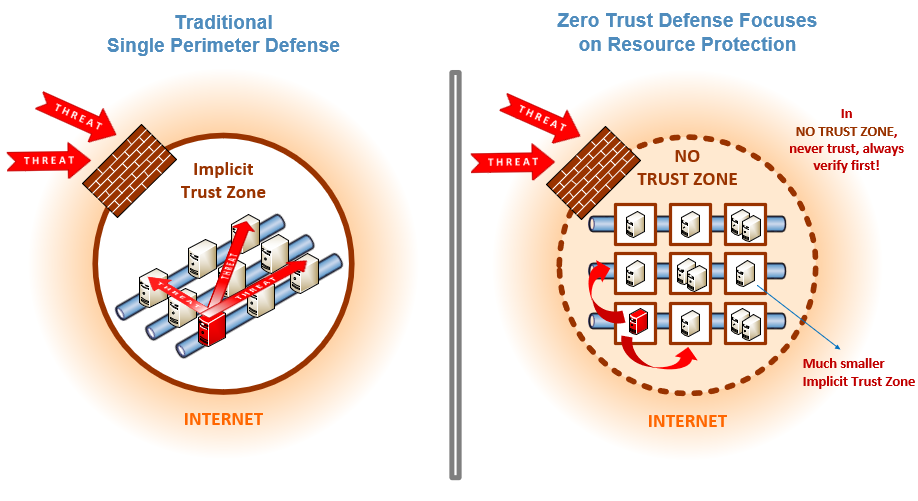
\includegraphics[width=\linewidth]{zero-trust.png}
\caption{Illustration of the difference between a traditional, firewalled network, which is vulnerable to East-West traffic and a network with zero-trust architecture.  (\url{https://www.techplayon.com/5g-reference-network-architecture/}).}
\Description{Illustration of the difference between a traditional, firewalled network, which is vulnerable to East-West traffic and a network with zero-trust architecture. }
\end{figure}

5G networks are characterized by high bandwidth, low latency, and massive connectivity, but these features also introduce greater security challenges, such as more complex attack surfaces and potential vulnerabilities, especially in large-scale IoT deployment scenarios. Each connected device can become a potential attack point, increasing the network's attack surface. The core network of 5G uses a SBA, which, while enhancing network flexibility and scalability, also introduces more interfaces and services, each potentially harboring vulnerabilities. Furthermore, the widespread adoption of Software Defined Networking (SDN) and Network Function Virtualization (NFV) technologies in 5G networks, which rely on software and virtual layers, could also become targets for attacks. The zero-trust architecture is crucial for these potential threats as it fundamentally changes the traditional network security model, moving away from reliance on perimeter defense and emphasizing strict scrutiny of every access request.

The mutual distrust model ensures that data is protected during every transmission process. The shift from traditional firewalled networks, which are vulnerable to East-West traffic, to networks employing zero-trust architecture marks a critical evolution in network security strategies, particularly relevant in the context of 5G networks where the scale and complexity of potential attack vectors are significantly expanded.

\subsection{Globally Unique Temporary Identifier}
To ensure the security and reliability of 5G networks, the network architecture incorporates multiple layers of security mechanisms, including user authentication, data encryption, and network access control. Among these, the GUTI plays a critical role in protecting user privacy by preventing the tracking of user location and identity information.

The IMSI (International Mobile Subscriber Identity) is a permanent and unique identifier for a subscriber within a cellular network, stored within the SIM card. Exposing the IMSI can lead to security vulnerabilities such as location tracking and eavesdropping \cite{3gpp23003}. To mitigate this risk, cellular networks do not transmit the IMSI over the open air interface; instead, they use a temporary identifier to mask the subscriber's identity. Prior systems like those before LTE used the TMSI (Temporary Mobile Subscriber Identity) for this purpose, while LTE and subsequent technologies use the GUTI \cite{goodin2013body}.

The GUTI comprises two main components: the Globally Unique Mobility Management Entity Identifier (GUMMEI) and the MME-Temporary Mobile Subscriber Identity (M-TMSI). The GUMMEI includes several identifiers for network identification, such as the Mobile Country Code (MCC), the Mobile Network Code (MNC), and the Mobility Management Entity ID (MME ID). The M-TMSI is a temporary and unique 32-bit value used specifically to identify a UE within an MME. An MME assigns a GUTI to a UE either when it first attaches to the network or when it updates its tracking area \cite{cheshire2015fake}.



\begin{figure}[htbp]
\centering
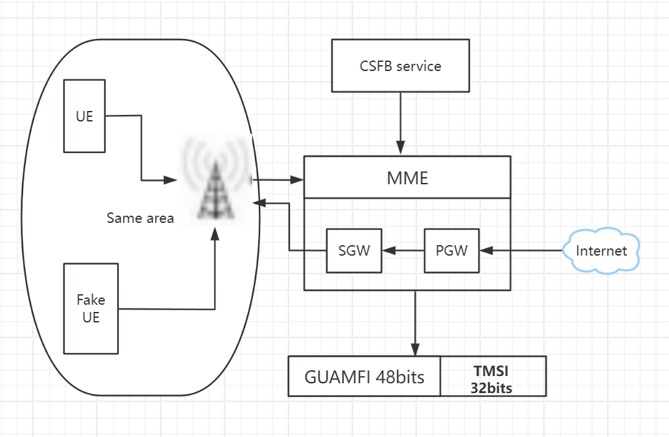
\includegraphics[width=\linewidth]{gutiAllocation.png}
\caption{The allocation process of GUTI.}
\Description{The allocation process of GUTI.}
\end{figure}

Following this assignment, the UE and the MME use the allocated GUTI for subsequent identification and communication activities, rather than the IMSI. To further obscure the mapping between subscribers and GUTIs, MMEs often reallocate GUTIs. The 3GPP standards do not specify the frequency or rules for this reallocation, thus it is typically determined by operator-specific configurations \cite{3gpp23003}. For example, a system implemented by Cisco may trigger GUTI reallocation based on the timing and frequency of access attempts. It can be configured to perform the GUTI reallocation procedure after every set number of ATTACH or TAU requests or periodically after a defined number of minutes \cite{hong2018guti}.

\section{Related Work}
This section describes previous works on preserving the privacy of mobile subscribers, highlighting the solutions and limitations found in current approaches.

\subsection{Developing Trust in 5G Network Slicing}
5G network slicing is a technology that partitions physical networks into multiple virtual network segments to provide differentiated services. Each network slice can independently satisfy specific service requirements \cite{jin2020research}. However, privacy protection faces many challenges in implementing this technology \cite{kholidy2022toward}. First, the multi-tenant environment of network slices requires high isolation and trust mechanisms between slices. Establishing trust becomes complex and unreliable due to the potential for slices to be operated by different service providers. Moreover, the diversity and complexity of slices increase the system's attack surface, making it easier for attackers to find vulnerabilities. Once a slice is breached, attackers can potentially move laterally to other slices, jeopardizing the entire network's security. Despite theoretically providing a flexible way to manage network resources, the actual application of network slicing has shown significant gaps in privacy protection.

\subsection{Enhanced Encryption Techniques and Increased Verification Processes}
Enhanced encryption and additional verification processes are common methods to protect data privacy, utilizing complex encryption algorithms and multi-factor authentication to secure data. However, these techniques have notable drawbacks in mobile network environments \cite{nie2022measuring}. Enhanced encryption often requires more computational resources and time, which can severely strain the capabilities of mobile devices and base stations. Additionally, increasing verification processes can add significant time costs to communication, which is detrimental in environments requiring high-speed data transmission. The maintenance costs are difficult to predict, making these methods impractical as a primary solution for mobile network privacy protection due to their high costs and complexity. 

\subsection{Use of VPNs}
Virtual Private Networks (VPNs) create secure channels over public networks to protect user privacy. While VPNs offer certain advantages in privacy protection, their applicability in mobile network environments has significant limitations. VPNs share network resources provided by Internet Service Providers (ISPs). Although different customers' VPNs are logically separated, the underlying infrastructure they use may be shared. This shared resource approach makes it challenging to strictly enforce Service Level Agreements (SLAs). For example, traffic from VPN 1 might interfere with VPN 2 when sharing the same infrastructure, impacting the SLA agreed upon with the ISP. In scenarios requiring a constant bit rate traffic between two sites on VPN 1, burst traffic from VPN 2 utilizing the same infrastructure could cause delays and packet loss \cite{makhija20235g}. Furthermore, VPNs often suffer from connection instability and slow speeds, negatively affecting the user's network experience. 


\section{Architecture Design}
Based on the examination of various solutions discussed in Section 3, we contemplate how to implement a Zero Trust model without impacting the existing 5G network models and standards.

\begin{figure}[htbp]
\centering
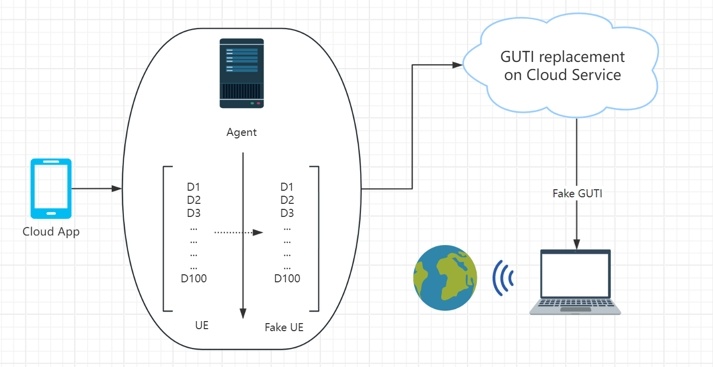
\includegraphics[width=\linewidth]{gutiAllocationApp.png}
\caption{The GUTI allocation on Cloud Service by Agent APP.}
\Description{The GUTI allocation on Cloud Service by Agent APP.}
\end{figure}

\subsection{Framework}
\paragraph{Step 1: Device Pool and Zero-Trust Control Logic}
We distribute devices across various geographic locations, each assigned a GUTI. A cloud-based zero-trust control logic manages these GUTIs, ensuring dynamic and secure distribution.
\paragraph{Step 2: Installation of the Zero-Trust APP}
Devices are equipped with the "Zero-Trust APP," a specially designed agent that interfaces with the cloud control logic to manage GUTI distribution effectively, enhancing user privacy without sacrificing performance.
\paragraph{Step 3: User Operation Flow}
Users activate zero-trust mode through the app, which selects GUTIs from the device pool based on the user’s region. This anonymizes network activities, such as web browsing, by substituting the user's actual GUTI with alternatives from the pool.
\paragraph{Step 4: Network Request Processing}
Network requests are anonymized by the Proxy APP, which replaces the user's GUTI with a randomly chosen one from the pool. This process is logged and randomized to maintain the integrity of the zero-trust model.
\paragraph{Step 5: Monitoring and Management}
The system continuously monitors the network and device pool, dynamically adjusting GUTI allocation policies to address privacy and security needs effectively.


\subsection{Methodology}
This section outlines the methodologies applied in the proposed Zero Trust Architecture for 5G networks, focusing on the establishment, allocation, and management of a GUTI pool, and the processes involved in ensuring robust privacy and security.

\subsubsection{GUTI Reallocation Mechanism}
Frequent invocation of the GUTI reallocation process can address privacy leaks due to GUTI persistence. However, this alone may not fully mitigate the issue \cite{kune2012location}. In LTE networks, GUTI reallocation is the primary procedure for changing GUTIs. According to 3GPP standards, GUTI reallocation can be triggered under the following conditions \cite{3gpp24301}:

\begin{itemize}
\item Network-initiated non-access layer "GUTI reallocation command."
\item When the UE attaches to the LTE network.
\item During a Tracking Area Update (TAU).
\end{itemize}

Given these triggers, our focus is on optimizing the GUTI reallocation process by utilizing a prepared "pseudo GUTI pool" for substitution. This approach is informed by methods discussed by Hong \cite{hong2018guti}, particularly using the Circuit Switched Fallback (CSFB) process as a trigger. Specifically, initiating a CSFB call forces a switch from LTE to 3G, releasing all LTE resources and requiring the device to reconnect to LTE, where a TAU triggers a GUTI reallocation.

Our solution for other network activities in 5G involves simulating common trigger conditions through a proxy APP to prompt GUTI reallocations. This includes programmatically disconnecting and reconnecting devices to the network to simulate an Attach process and using VPN services to change IP addresses, simulating TAU at the network level.

\subsubsection{Establishment of the GUTI Pool}
The GUTI pool is structured according to the geographical architecture of the network, with each TA identified by a unique TAC. The MME manages subscriber locations by integrating the TAC with the MMEC. This structure prevents authentication conflicts arising from inconsistencies between TAC and MMEC codes within different TAs \cite{hong2018guti}.

\subsubsection{GUTI Replacement Process}

\begin{figure}[htbp]
\centering
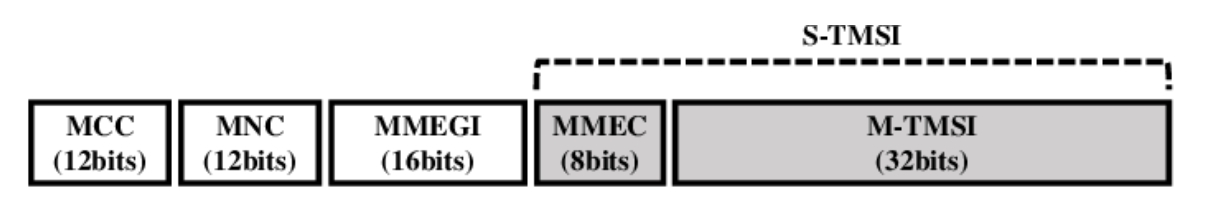
\includegraphics[width=\linewidth]{gutiStructure.png}
\caption{The Structure of the GUTI.}
\Description{The Structure of the GUTI.}
\end{figure}

Upon accessing the network and obtaining a GUTI, the UE’s data is sent to a cloud-based server that handles the replacement logic. This ensures no sensitive user data is stored locally, enhancing security. The process involves replacing the M-TMSI component of the GUTI—responsible for user identification within the network without exposing permanent identity—while maintaining other components constant for compatibility with legacy systems \cite{3gpp23003}.

The remaining components are the MMEC, the public land mobile network codes (MCC and MNC) and the MME Group ID, which can be considered constant. We also ignore the MMEC, which may be changed in the GUTI reallocation by the operator using the MME pool \cite{hong2018guti}.

\subsubsection{Security and Privacy Measures}
Our system continuously monitors network conditions to quickly respond to fluctuations or outages. Upon detecting instability, it immediately terminates all sessions and severs network connections to safeguard against data breaches. All sensitive data stored temporarily is securely erased, ensuring no residual information is left vulnerable.

Data security is enforced through advanced encryption using cryptographically secure pseudorandom number generators (CSPRNGs). These generators, unlike standard PRNGs, produce sequences that are computationally unpredictable, ensuring the confidentiality and integrity of data during transmission \cite{soto1999statistical}. The encryption process is supported by robust algorithms like Hash\_DRBG, which generates bits from a high-entropy seed, rendering the output undecipherable to unauthorized entities \cite{barker2016nist}.

GUTI replacements are performed on highly secure cloud servers, shielded from external threats and monitored continuously. Operations undergo strict access control and comprehensive logging to maintain security and accountability. At the end of each session, the system ensures that no user data remains stored, preserving user privacy by immediately erasing all identity-related information.

\section{Implementation}
Given the complexity of our architecture, this project utilizes TCP sockets to simulate the GUTI pseudonym system and Zero Trust process in Python 3.12. The client represents the UE and the server acts as the network end, managing communication and GUTI concealment.

\subsection{Simulation}

\begin{figure}[htbp]
\centering
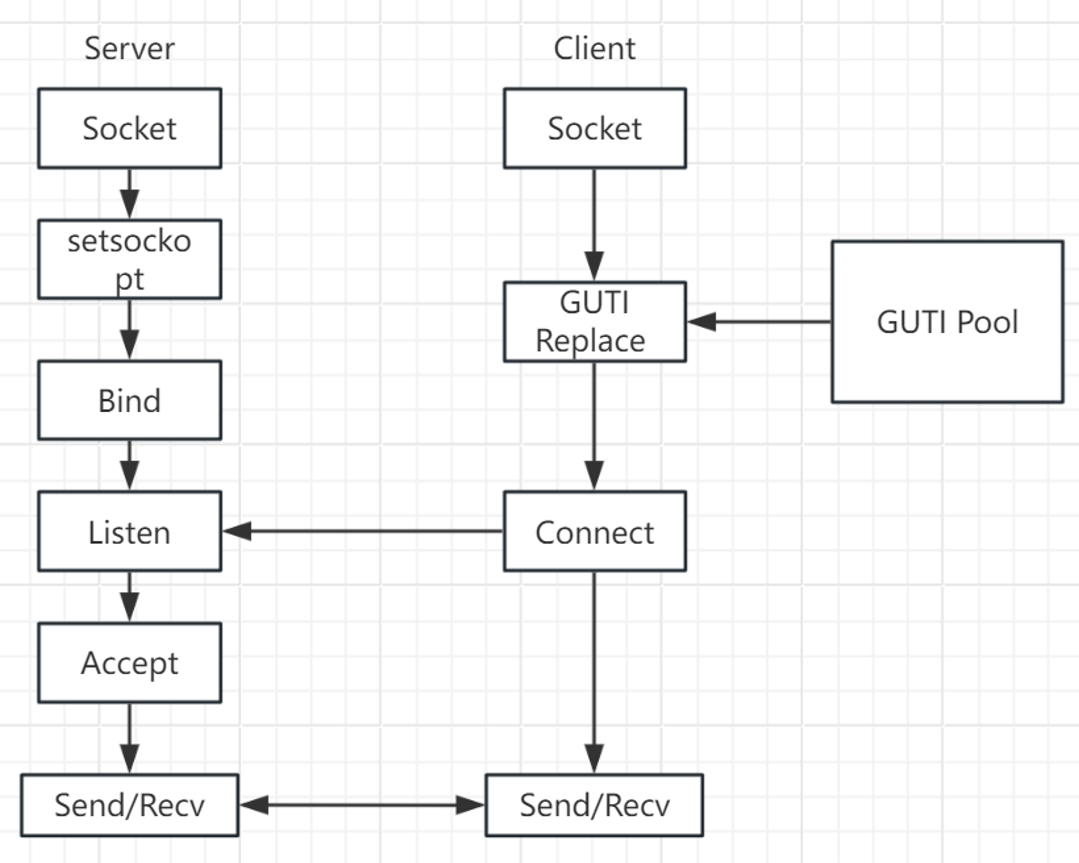
\includegraphics[width=\linewidth]{implement.png}
\caption{The client side and the server side serve as the basis to implement the TCP socket function system implementation structure diagram.}
\Description{The client side and the server side serve as the basis to implement the TCP socket function system implementation structure diagram.}
\end{figure}

Initially, we set up the client and server to support basic TCP socket functionality. We simulate a GUTI pool with random number combinations that share the first two digits, representing UEs in the same tracking area. When a UE activates Zero Trust mode, the client allocates an available GUTI from the pool and applies a replacement strategy before initiating communication.

The client sends a request to connect with the server, allowing users to transmit customizable information (simulating web browsing). When the server receives this data, it displays the GUTI, which has been replaced by then, thus recognizing communication with a pseudonymized user. This setup effectively demonstrates the practical application of hiding real user identifiers under the Zero Trust model, enhancing privacy and security during network interactions.

\subsection{Performance and Evaluation}

\begin{figure}[htbp]
\centering
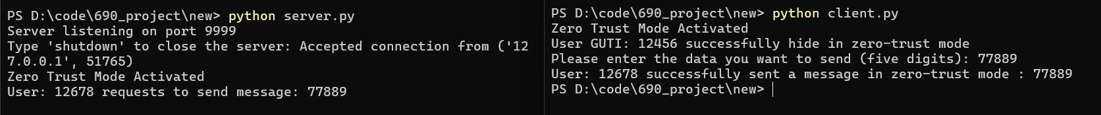
\includegraphics[width=\linewidth]{gutiCode.png}
\caption{The process in which the client randomly selects GUTI and replaces it.}
\Description{The process in which the client randomly selects GUTI and replaces it.}
\end{figure}

As demonstrated in Figure 8, the client randomly selects a GUTI (12456) from the pool and successfully masks it under Zero Trust mode. Upon entering a five-digit data packet (77889), the system replaces the GUTI with 12678 before sending it to the server. This ensures that the server cannot recognize the user's real identity, thus showcasing the effectiveness of the GUTI transformation mechanism in protecting user privacy. The server receives and processes the data packet from the pseudonymized user (12678) without knowing the user's actual GUTI. This confirms that our system can effectively protect user privacy during data transmission, aligning with the Zero Trust architecture's objectives.

\begin{figure}[htbp]
\centering
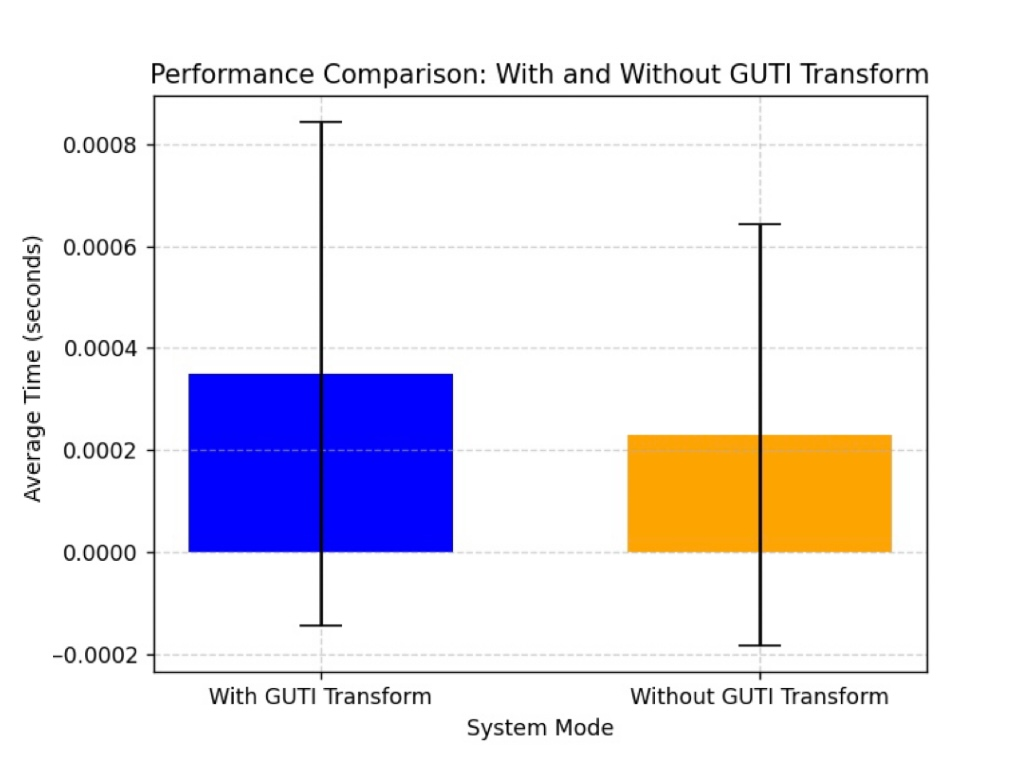
\includegraphics[width=\linewidth]{performanceComparison.jpg}
\caption{The Performance Comparison when with and without GUTI Transform.}
\Description{The Performance Comparison when with and without GUTI Transform.}
\end{figure}

We conducted a systematic evaluation using a Python script to test two scenarios: systems with a GUTI transformation function and systems without it. Under the conditions of 20 random GUTIs, we performed 50 consecutive TCP socket communications and assessed the overall and individual response speeds.

\begin{figure}[htbp]
\centering
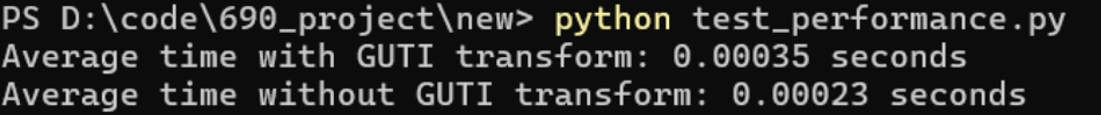
\includegraphics[width=\linewidth]{averageTime1.png}
\caption{Average Time with and without GUTI Transform.}
\Description{Average Time with and without GUTI Transform.}
\end{figure}

The results indicate that the average time for GUTI-transformed systems was 0.00035 seconds, compared to 0.00023 seconds for non-GUTI-transformed systems. Although the inclusion of GUTI transformation introduces a slight processing overhead, the actual impact is minimal, making the additional time cost negligible when our Zero Trust system is enabled.

\begin{figure}[htbp]
\centering
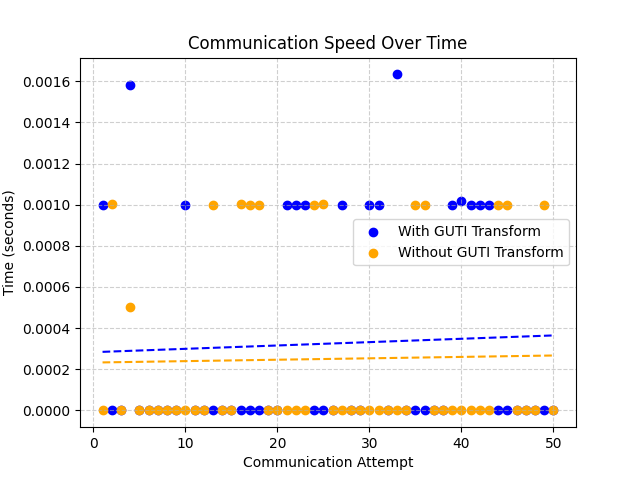
\includegraphics[width=\linewidth]{communicationSpeed.png}
\caption{The Communication Speed of GUTI converted systems and Non-GUTI converted systems across multiple attempts.}
\Description{The Communication Speed of GUTI converted systems and Non-GUTI converted systems across multiple attempts.}
\end{figure}

The communication times for both GUTI-transformed and non-GUTI-transformed systems across multiple attempts show that while non-GUTI-transformed systems display more consistent and stable communication times, the GUTI-transformed systems exhibit initial fluctuations but stabilize over time. The average time taken by GUTI-transformed systems is slightly higher, but as communication attempts increase, the time required tends to align closely with that of non-GUTI-transformed systems, proving the system’s feasibility and stability.

\begin{figure}[htbp]
\centering
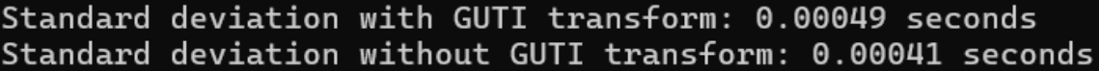
\includegraphics[width=\linewidth]{standardDeviation.png}
\caption{The Standard Deviation of GUTI converted systems and Non-GUTI converted systems across multiple attempts.}
\Description{The Communication Speed of GUTI converted systems and Non-GUTI converted systems across multiple attempts.}
\end{figure}

We also measured the variability of communication times by calculating the standard deviation for each mode. A larger standard deviation indicates greater variability in communication times. It can be seen from the standard deviation results that the communication time of GUTI converted systems has larger fluctuations and larger standard deviation. The communication time of Non-GUTI converted systems has less fluctuation and smaller standard deviation. The difference in mean standard deviation is 0.00008. This shows that the communication time of Non-GUTI converted systems is more stable, but the stability difference between the two systems is not big and can be ignored.

\begin{figure}[htbp]
\centering
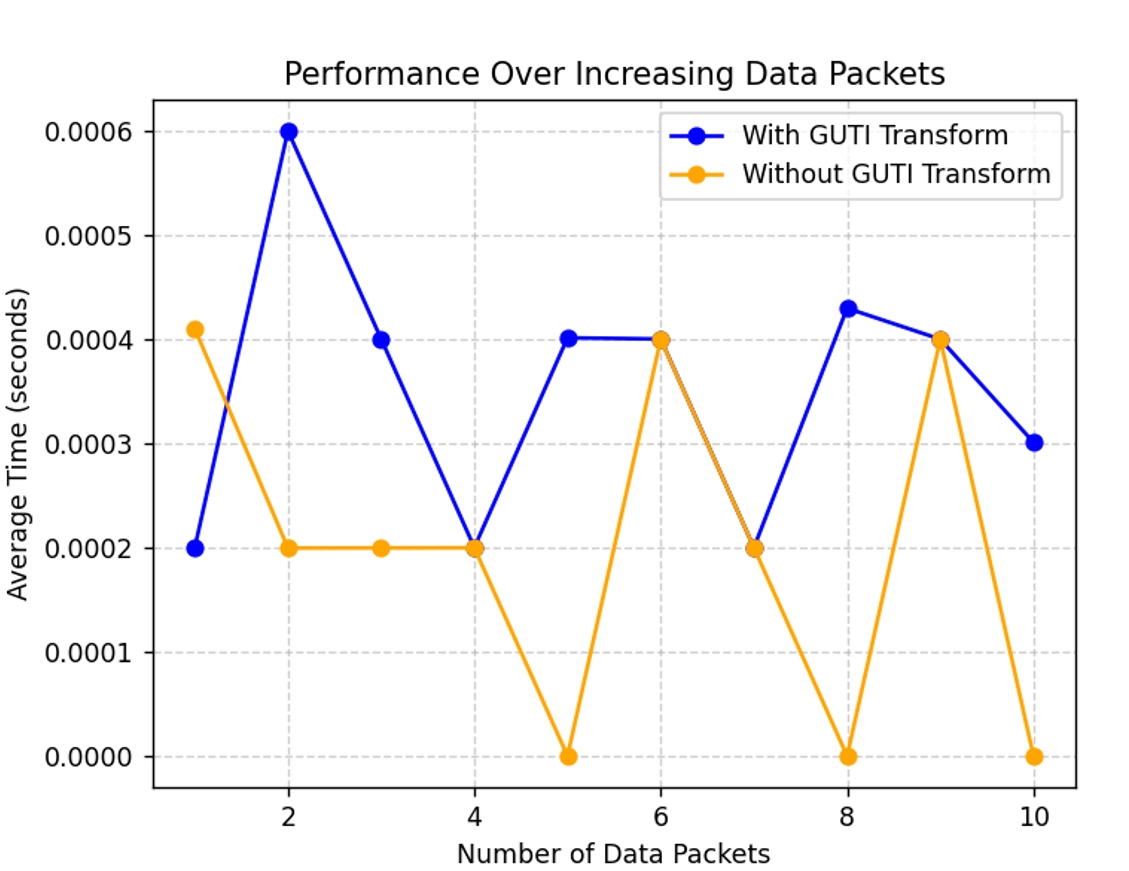
\includegraphics[width=\linewidth]{performanceIncrease.png}
\caption{The average time it takes for dual systems to transmit one data packet to ten data packets five times each.}
\Description{The average time it takes for dual systems to transmit one data packet to ten data packets five times each.}
\end{figure}

\begin{figure}[htbp]
\centering
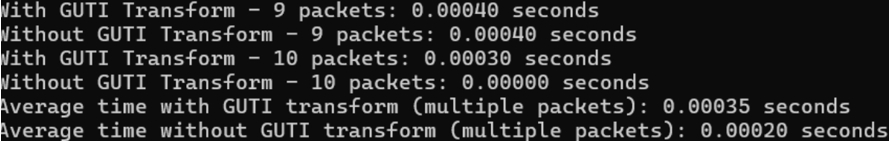
\includegraphics[width=\linewidth]{averageTime2.png}
\caption{Average Time with and without GUTI Transform to transmit one data packet to ten data packets five times each.}
\Description{Average Time with and without GUTI Transform to transmit one data packet to ten data packets five times each.}
\end{figure}

Further testing on the performance impact of transmitting multiple data packets revealed that while GUTI-transformed systems consistently took slightly longer, the highest difference was only 0.0004 seconds, with an average difference of just 0.00015 seconds—both at the microsecond level.

These tests confirm that enabling GUTI transformation has a very small impact on communication times. The minor increase in average time and comparable stability demonstrate the viability and superiority of our system architecture.


\section{Conclusion}
In this study, we proposed a GUTI-based pseudonym system as a solution by learning and researching the application of zero-trust architecture in 5g networks. This architecture designs a pseudonym system from hardware to software, from the user side to the 5G network side. By replacing and hiding the GUTI, it implements a zero-trust model and enhances user privacy and data security. The proposed system has implications for the inherent security challenges posed by the open and decentralized nature of 5G networks.

Performance evaluations affirmed the system's efficiency, showing minimal impact on latency despite the computational demands of GUTI transformations. The results confirmed that our architecture supports stable communication speeds and efficiently manages data transmission, aligning with Zero Trust security requirements without compromising performance.

\section{Future Works}
\paragraph{Integration with Open5G Cloud Servers:}
We plan to integrate the GUTI-based pseudonym system with Open5G servers, using UERANSIM to more effectively simulate real UE and base station communications. This step will refine the Zero Trust APP and test its effectiveness in realistic 5G environments.
\paragraph{Development and Optimization:}
Continuous development is needed to align our system with 5G standards and cloud protocols. We will address technical challenges identified in initial testing to improve robustness, scalability, and prepare for academic publication.
\paragraph{Deeper Analysis of Anomalies:}
Initial tests indicated promising results but also presented anomalies, such as irregular performance spikes in GUTI-converted systems. Further investigation will focus on understanding and resolving these issues to ensure system stability and efficiency.


\bibliographystyle{ACM-Reference-Format}
\bibliography{main}


\end{document}
